\documentclass{MO_article}
\usepackage{amsmath}
\usepackage{amssymb}
\usepackage{caption}
%\usepackage{palatino}

\title{Dynamo: \\
 The design, data model and implementation of the GungHo dynamical core for the Met Office.}
\author{The LFRic Team}

\date{\today}

\begin{document}

\maketitle

\section{Abstract}

Dynamo is the software infrastructure for the Met Office
implementation of the GungHo dynamical core, and is a prototype for
the infrastructure for the future LFRic atmosphere model that is
intended to replace the Unified Model during the 2020s. 

The Dynamo design follows recommendations from the GungHo project
\cite{gunghocs} (formally known as ``the Next Generation Weather and
Climate Project''). The GungHo project was a joint project between the
Met Office, NERC-funded universities and STFC. The collaboration
continues as an ongoing networking activity. It has delivered both a
scientific formulation for the dynamical core and a high-level
software design. The design aims to ensure that the dynamical core is
scalable on future HPC architectures, and seeks to apply a separation
of concerns between science and computational science aspects of the
model. The design relies on part of the Dynamo code being generated by
a complementary tool called PSyclone.

This document describes how the scientific requirements of the GungHo
dynamical core feed into the software design of Dynamo. Following
this, the Dynamo design and data model are discussed in more detail.

\section{Introduction}

The GungHo project is a research collaboration between the Met
Office, NERC-funded researchers and STFC Daresbury to design a new
dynamical core that will exhibit very large data parallelism.

The GungHo dynamical core will use the Finite Element Method
(FEM). FEM is a standard method used in many modelling applications,
and there are many software packages and standards that are available
to support the development of FEM codes. The GungHo requirements mean
that many of these packages and standards do not quite fit. They
include the need to support higher order finite element methods, the
choice of a mixed finite element scheme, and the need to support a
mesh that is unstructured in the 2D horizontal atmospheric fields but
structured in the vertical. These requirements are discussed in more
detail in this document.

The GungHo computational science recommendations relate to the design
of the science modules, referred to as the ``single model
design''. The GungHo design is nicknamed {\em PSyKAl}. It separates
the concerns of scientists writing scientific {\em K}ernels and {\em
  A}lgorithms from the concerns of engineers and computer scientists
optimising the {\em P}arallel {\em Sy}stems layer (PSy-layer) that
supports execution of the code.

The implementation of the design uses metadata to describe the
algorithms and kernels such that the Parallel Systems layer can be
automatically generated for different HPC architectures and different
optimisation requirements.

This document will discuss these concepts and designs in more detail,
and will then describe the implementation of the GungHo design for Met
Office use. The implementation comprises two applications called
Dynamo and PSyclone. They are being developed by the Met Office, STFC
Daresbury and the University of Manchester.

\section{The Mesh and Topology}
\subsection{Unstructured meshes in two dimensions}

\label{sec:meshSec1}

The terminology for describing the GungHo grid derives from other
scientific fields that use the term ``mesh'' rather than ``grid''. The
term ``mesh'' is therefore used in this document.

In longitude-latitude (lon-lat) models such as the UM, lines of
longitude and latitude are used to construct the mesh used to
discretise the equations describing the behaviour of the
atmosphere. Such a mesh is described as {\em structured} as it aligns
well with native computational data array structures (such as 2D or 3D
arrays of real numbers in Fortran or C).

The structure of the mesh makes it relatively easy to code
computations on mesh cells that are dependent on neighbouring cells.
\begin{itemize}
\item The cells to the east and west are next to the cell in memory
  whereas those to the north and south are obtained by subtracting or
  adding the number of cells in an east-west row.
\item Geographical information can be computed by knowing the row and
  column number of the cell relative to some fixed point.
\end{itemize}

Global model configurations that use the lon-lat mesh suffer from
numerical and performance problems where the mesh cells converge at
the north and south poles. These problems will grow as the model
resolution increases, and they will limit the scalability of the model
on large numbers of compute cores. See \cite{buckeridge} for a
discussion.

The GungHo project developed a formulation that can be implemented on
spatially uniform meshes without such convergence of cells. Examples
of such meshes include a cubed-sphere mesh and a mesh comprising a
tessellation of hexagons and pentagons (see
Figure~\ref{fig:icosahedron}). Such global meshes are referred to as
being ``semi-unstructured'' as the total mesh has structure but one
which does not map onto standard computer programming data structures
in an obvious way.

Such a mesh requires a more explicit description within the code than
a regular lon-lat mesh, to describe relationships between neighbouring
cells of the mesh and to describe their location.

% An unstructure Mesh
\begin{figure}
\centering
\resizebox{0.66\linewidth}{!}{
 \includegraphics*{truncatedIcosahedron.eps}}
\caption{A truncated icosahedron}
\label{fig:icosahedron}
\end{figure}

A mesh is described by coordinates of a set of points called
``vertices'', and a topology defined by the list of connections
between pairs of vertices. A polyhedral 2-dimensional mesh, such as a
cubed-sphere or truncated icosahedron (see
Figure~\ref{fig:icosahedron}), can be projected onto a sphere. Each
face of the polyhedron can be treated as a two-dimensional cell. We
define three separate ``mesh entities'' for such a 2D mesh:

\begin{itemize}
\item Vertices, which are points of zero dimension.
\item Edges, which are the lines connecting vertices, and which define
  the topology of the mesh;
\item Cells, which for the meshes we are considering, are the surfaces
  of the sphere enclosed by a set of edges projected onto the sphere.
\end{itemize}

Depending on the needs of a scientific formulation, a field
representing a physical quantity such as temperature or potential
vorticity may be described by storing data associated with vertex
points, edges or cells, or with a combination of entities. For
example, a data value on an edge may define the flux of a quantity
between the cells either side of it. In the computer memory, the
values that represent a field can be stored in an array such as a
one-dimensional array of real numbers. To relate a particular element
or set of elements of the array to a particular vertex, edge or cell
entity there must be an agreed mapping between the field array and the
data values associated with each of the mesh entities. Unlike a
lon-lat mesh, where one can compute the location of a cell from its
position in the data array and vice versa, a semi-unstructured mesh
will not have an obvious or implicit ordering of entities.

% A numbered hexagonal mesh

\begin{figure}
\centering
\resizebox{0.66\linewidth}{!}{
 \includegraphics*{numberedHexMesh.eps}}
\caption{A hexagonal mesh numbered to store fields whose values are
  defined on cells and fields whose values are defined on
  vertices. Vertices are numbered from 1 to 28. Cells are numbered
  from C1 to C8. In principle the order of numbering is arbitrary,
  though the choice can affect run-time performance.}
\label{fig:numberedHexMesh}
\end{figure}

Look-up arrays are required to relate an element of a data field to
the specific entity in the mesh that it relates
to. Figure~\ref{fig:numberedHexMesh} illustrates the numbering of the
cells and the vertices of a hexagonal mesh. A two-dimensional array
can be computed that lists the vertex numbers for each of the
hexagons. In the following array, the row number relates to the cell
number {\tt C1} to {\tt C8}, and the 6 numbers in each row number the
vertices of each hexagon in an anti-clockwise direction.

\[ lookup(vertex\_number, cell\_number) = \left\{ \begin{array}{cccccc} 
1 & 2 & 3 & 4 & 5 & 6 \\
10 & 6 & 5 & 7 & 8 & 9 \\
3 & 11 & 12 & 13 & 14 & 4 \\
5 & 4 & 14 & 15 & 16 & 7 \\
14 & 13 & 17 & 18 & 19 & 15 \\
16 & 15 & 19 & 20 & 21 & 22 \\
17 & 23 & 24 & 25 & 26 & 18 \\
19 & 18 & 26 & 27 & 28 & 20 \\
\end{array} \right\} \]

Consider a field which has data points on each of the 28 vertices, and
a field that has data points on each of the 8 cells. To compute
changes to the first field that are a function of the second, one can
loop over all the cells. To do so one can construct a loop over all
choices of cell number {\tt C1} to {\tt C8}. Within this loop over
cells, an inner loop is required to loop over the values of the
field. The inner loop loops over the numbers in the row for that cell
number to get the address of the value in the field array.

\begin{verbatim}
do cell = 1, number_of_cells
  ! Get the value of the cell field for this cell
  value = field_on_cell(cell)

  ! Loop over all vertices 
  ! Note some cells may have a different number of vertices
  do vertex = 1,vertex_on_cell(cell)
    ! Update each increment depending on the cell value
    call operation( value, field_on_vertex(lookup(cell,vertex) )
  end do
end do
\end{verbatim}

\subsection{Vertical Levels and Extruded Meshes} 
In current atmosphere models, the two dimensional mesh is extruded
into three dimensions by replicating the mesh over a number of layers
such that each 2D lon-lat cell becomes a column of 3D cells.

Due to the curvature of the Earth, the columns get wider as you go up
from the surface (see Figure~\ref{fig:cubedSphere}. Layers can be of
different thickness: it is common for atmosphere models to have layers
near the Earth's surface that are thinner than those higher
up. Heights of layers can be nominal values that follow terrain of the
orography, or that are related to surface pressure.

% A 3D cubed-sphere mesh
\begin{figure}
\centering
\resizebox{0.66\linewidth}{!}{
 \includegraphics*{cubed_sphere.ps}}
\caption{A 3-dimensional cubed sphere mesh, taken apart to see the
  levels structure}
\label{fig:cubedSphere}
\end{figure}

In many computational fluid dynamics application, the mesh is
unstructured in three dimensions. Coordinates and connectivity of the
whole mesh need to be explicitly stored. In atmospheric model
applications, however, it is usual to define a mesh in which every
layer has vertices on the same set of latitude and longitude points,
and GungHo will follow this pattern. Therefore one need only store the
coordinates and connectivity information for a single horizontal level
of vertex points, and infer coordinates of all levels from this
information plus a list of height coordinates.

The extrusion of the 2D mesh into a 3D mesh {\tt n} cells deep
requires us to extend and vary the list of mesh entities. We now have:

\begin{itemize}
\item Vertices - a vertical column of vertices all at the same
  latitude and longitude of the 2D mesh.
\item Edges:
 \begin{itemize}
 \item There are vertical edges which connect the vertices with the
   same latitude and longitude on each adjacent height level.
 \item There are horizontal edges which connect vertices as in the 2D
   example on each layer of the 3D mesh.
 \end{itemize}
\item Faces
 \begin{itemize}
 \item There are vertical faces which are the 2D faces between an edge
   on one height level and the corresponding edge on the next.
 \item There are horizontal faces which are as the original 2D
   faces/cells description except there is a set of horizontal faces
   on each level.
 \end{itemize}
\item Cells are 3D elements created by the extrusion of the 2D
  face into 3D. 
\end{itemize}

\subsection{Mapping the field data structures}

Physical fields are described in the GungHo model by data points
mapped onto the mesh. The GungHo model uses several different mappings
some of which are illustrated in Figure~\ref{fig:k0k1w0-w3}.

A field made up of cells like those in Figure~\ref{fig:k0k1w0-w3}b has
a data point associated with every vertex, edge, face and cell. It
therefore provides a good example of the GungHo recommended
field-mapping strategy. 

A typical operation on a field loops over each cell in turn. Each
iteration of the loop operates on all data points touched by a
cell. In the example field, each cell touches 27 data points (8 vertex
points, 12 edge points, 6 face points and one in the cell body). In
the full field, the data points on the faces, edges and vertices are
touched by more than one cell.

As discussed in Section~\ref{sec:meshSec1}, the addresses of the data
points relating to each cell of a single horizontal level of the field
can be specified by a look-up array. There remains the question of how
to structure the data to represent the field in the vertical.

% A section of a 3D mesh Mesh
\begin{figure}
\centering
\resizebox{0.66\linewidth}{!}{
 \includegraphics*{w0_3d_full.eps}}
\caption{Numbering of the data points representing a field of the type
  shown in Figure~\ref{fig:k0k1w0-w3}b. For simplicity, just two
  columns of a larger 3D mesh are shown, and the numbering of values
  for points hidden behind the cells is not shown.}
\label{fig:Mesh}
\end{figure}

The atmosphere models being considered will use a mesh with the same
number of cells in the vertical at every location. Each cell is
associated with the same number of data points in the same relative
locations. It is therefore possible to number the data points such
that the address of the data points associated with a cell on layer
{\tt n} where {\tt n > 1} can be obtained by adding 1 to the addresses
of the values of the cell on the level below. By doing this, one need
only store the look-up array that addresses cells on the lowest
level. One can construct a loop over the number of levels, and address
the cell on each level in turn by adding one to the addresses of the
data points in the lowest level for each loop iteration. Such loops
may be able to make good use of memory cache lines as the data in a
column of cells is represented by several blocks of data that is
contiguous in memory \cite{macdonald}.

Figure~\ref{fig:Mesh} illustrates this way of numbering data points.
For simplicity, it illustrates just two columns of a larger 3D mesh
that has 3 levels. The ordering of numbering of the individual columns
is done in an arbitrary way in this example. In a real field there may
be an optimal method of numbering points that gives performance
benefits due to better memory use.

For clarity of the image, only the numbering on the visible sides of
the cells are shown. As some of the data points in the image are
hidden, a description of the ordering follows to help to explain the
numbers at the top of the column.

The data points on each of the 4 vertices of the bottom left cell are
numbered in a clockwise order (looking from above). This is why the
vertices of the cells at the top cell are numbered 4, 8, 12, 16. Next
to be numbered are the data points on the vertical edges (starting
with 17), then horizontal edges starting with 29, then vertical faces
starting with 45, then the horizontal face (number 57 situated on the
base below 60) then the data points within the cell volume (numbered
61, but none of the data points in the cell volume are shown in the
illustration).

Numbering of the data points of the second cell follows the same order
for those cells that are not shared with the first cell.

The look-up array that addresses the 27 points of the base cells of
these two cells are therefore as follows (not every number is shown):

\[ lookup = \left\{ \begin{array}{ccccccccccccccccccc} 
1 & 5 & 9 & 13 & 2 & 6 & 10 & 14 & 17 &  20 & 23 & \ldots & 45 & 48 & 51 & 54 & 57 & 58 & 61 \\
5 & 64 & 68 & 9 & 6 & 65 & 69 & 10 & 20 & 72 & 75 & \ldots & 90 & 93 & 96 & 48 & 99  & 100 & 103 \\
\end{array} \right\} \]

Entirely different numbering strategies could be followed for some
fields while still maintaining a consistent relationship between cells
on subsequent levels of a field. For example, in some types of field
no data points are shared between neighbouring cells. Therefore, one
can number all the data points in a cell sequentially. For example,
the field made up of cells like those in Figure~\ref{fig:k0k1w0-w3}d
has 8 points in the body of each cell. Each point is nominally
situated at the vertex, but the neighbours each have their own data
point for the same vertex. If data points are numbered this way, then
the cell at the base could have data points 1-8 in the field array,
the cell above has data points 9-17, and so forth. Rather than adding
1 to the addresses of the data points at the base level to get the
address of the points at subsequent levels, one needs to add a number
corresponding to the number of points per cell: in this case 8.

For operations on cells of fields of this latter type, this data
layout may be more efficient as data for the whole cell is contiguous
in memory. However, the GungHo mixed finite element formulation mixes
fields of all the types as shown in Figure~\ref{fig:k0k1w0-w3}. Mixing
and matching numbering strategies adds complexity to the
infrastructure. Initially, the Dynamo implementation will use the same
strategy for all fields.

\section{The Finite Element Method}

The GungHo dynamical core will use the Finite Element Method. This
document proposes to describe only those aspects of the Finite Element
Method (FEM) that are required to understand the design of Dynamo.

\subsection{Representation of fields in FEM}

In the Finite Difference method (as commonly used in atmosphere models
such as the Unified Model) fields are represented as discrete values
at particular locations of the mesh. For example, in the Arakawa-C
mesh, mass fields are represented by values at the centre of cells,
and vector fields by values located on the edges of cells.

In FEM, fields are additionally represented by spatial functions in a
{\em function space} rather than as discrete values. Essentially, the
value of a field at any point within a cell is defined by the sum of a
set of spatial functions multiplied by coefficients which are the data
points. The functions are called {\em basis functions}. 

In FEM, each data point or coefficient is called a {\em degree of
  freedom} or {\em dof} for short. Every cell in a given field has the
same set of basis functions. Different fields may have a different
function space and therefore a different set of basis functions.

A field therefore comprises the field of data points, referred to as
the degrees of freedom, and a reference to the function space. The
actual value of a field $f$ at point $x,y,z$ within a cell can be
given as:

\[ f(x,y,z) = \sum_{i=1}^n x_i \sigma_i(x,y,z) \] 

where $\sigma_n$ are the basis functions, $x_n$ are the values of the
degrees of freedom and $x,y,z$ is a relative position within the cell
to take account of the fact that cells can be of different sizes.

Some fields are constant within each individual cell, in which case
just one dof per cell is required to describe the field. A scalar
field that varies linearly throughout an n-dimensional cell
(``piecewise linear'') requires $2^n$ degrees of freedom. A bilinear
field requires $3^n$ degrees of freedom and so forth.

Note that we have now introduced the concept of multiple degrees of
freedom per mesh entity. This concept will be discussed in more detail
in the Section~\ref{sec:higherOrder}.

\begin{figure}
\centering

\begin{minipage}{.4\textwidth}
  \centering
  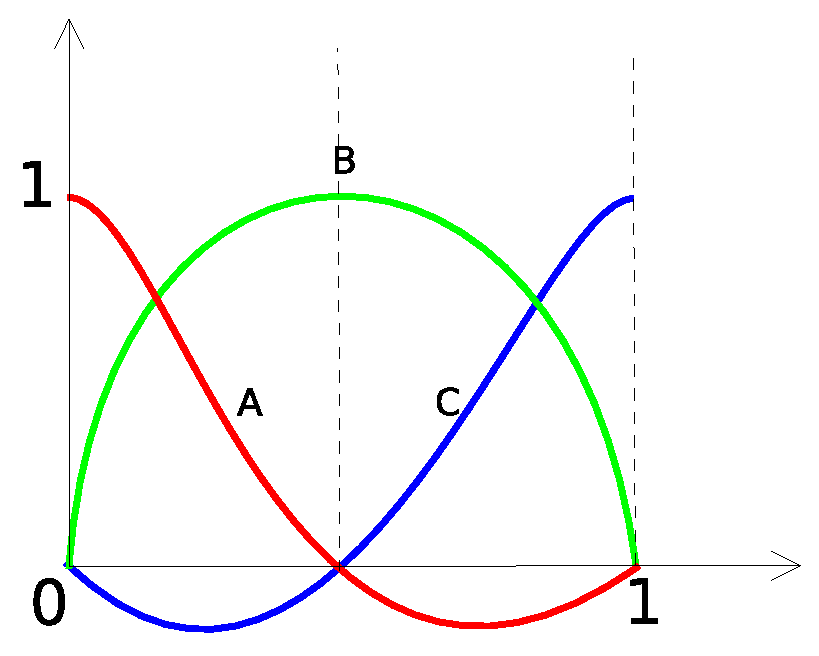
\includegraphics[width=1.0\linewidth]{basisOrder2.eps}
  \caption*{a) Basis functions}
\end{minipage}%
\begin{minipage}{.4\textwidth}
  \centering
  \includegraphics[width=1.0\linewidth]{basisOrder2_dofs.eps}
  \caption*{b) Degrees of freedom}
\end{minipage}

\begin{minipage}{0.7\textwidth}
  \centering
  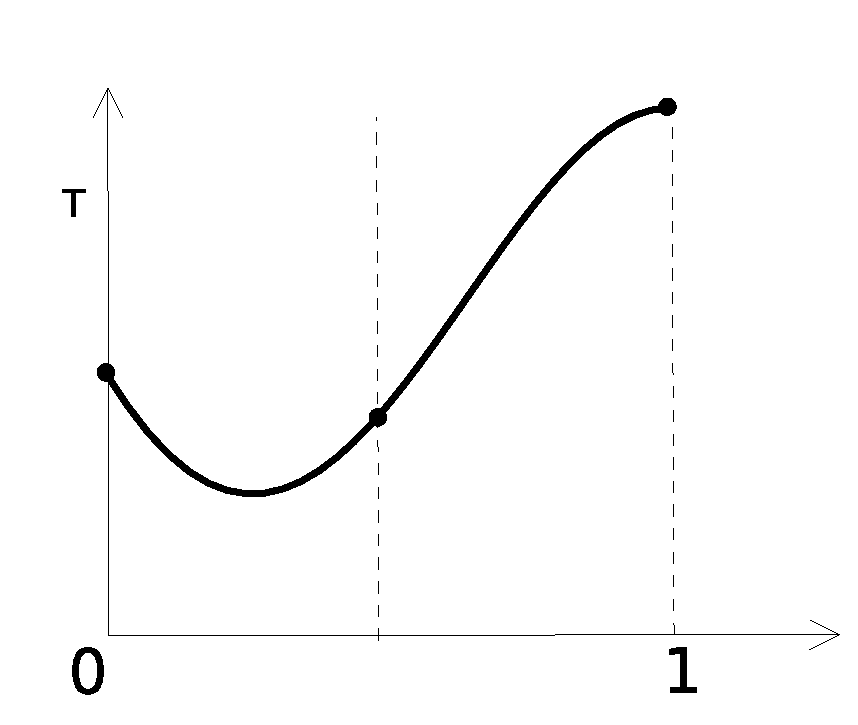
\includegraphics[width=0.8\linewidth]{basisOrder2_field.eps}
  \caption*{c) Field value superimposed on the dof values from Figure b)}
\end{minipage}
  \caption{Multiplying each basis function in Figure a) (labelled A, B
    and C) by the value of its related dof in Figure b) (from left to
    right) gives the sum displayed by Figure c). Note that the sum
    intersects all three dofs as at the locations of the dofs, one of
    the basis functions is of value 1 and the other two are zero.}

\label{fig:basis_function}
\end{figure}

Basis functions are usually chosen such that for each of the basis
functions, there is one location in the entity which each of the basis
functions is equal to 1 and all other functions (if there are more
than one) are zero. Therefore, the value of the dof is equal to the
value of the field at the location of the dof. To illustrate,
Figure~\ref{fig:basis_function} shows how basis functions for a
one-dimensional field are combined with the dof values to give the
field value within the cell.

\subsection{Continuous and Discontinuous fields}

\label{sec:continuity}

A field can be continuous or discontinuous across the boundary between
two cells. Figure~\ref{fig:differentContinuity1D} shows examples of a
quadratic field in one dimension, and shows locations of the degrees
of freedom. If a field is discontinuous across a boundary then each of
the cells requires its own set of dofs to define the field within the
cell. In this case, 3 dofs per cell are required. However, if there is
continuity across the boundary, then dofs in one cell can be shared
with dofs in the neighbouring cell in a way that guarantees that the
value of the field just either side of the boundary between cells is
identical.

A field can have mixed continuity, for example, it may be continuous
in one direction (e.g. in the horizontal), but discontinuous in
another (e.g. in the vertical). Vector fields may have components that
are continuous normal to a face between two cells, but are
discontinuous parallel to the face.

\begin{figure}
\centering

\begin{minipage}{.5\textwidth}
  \centering
  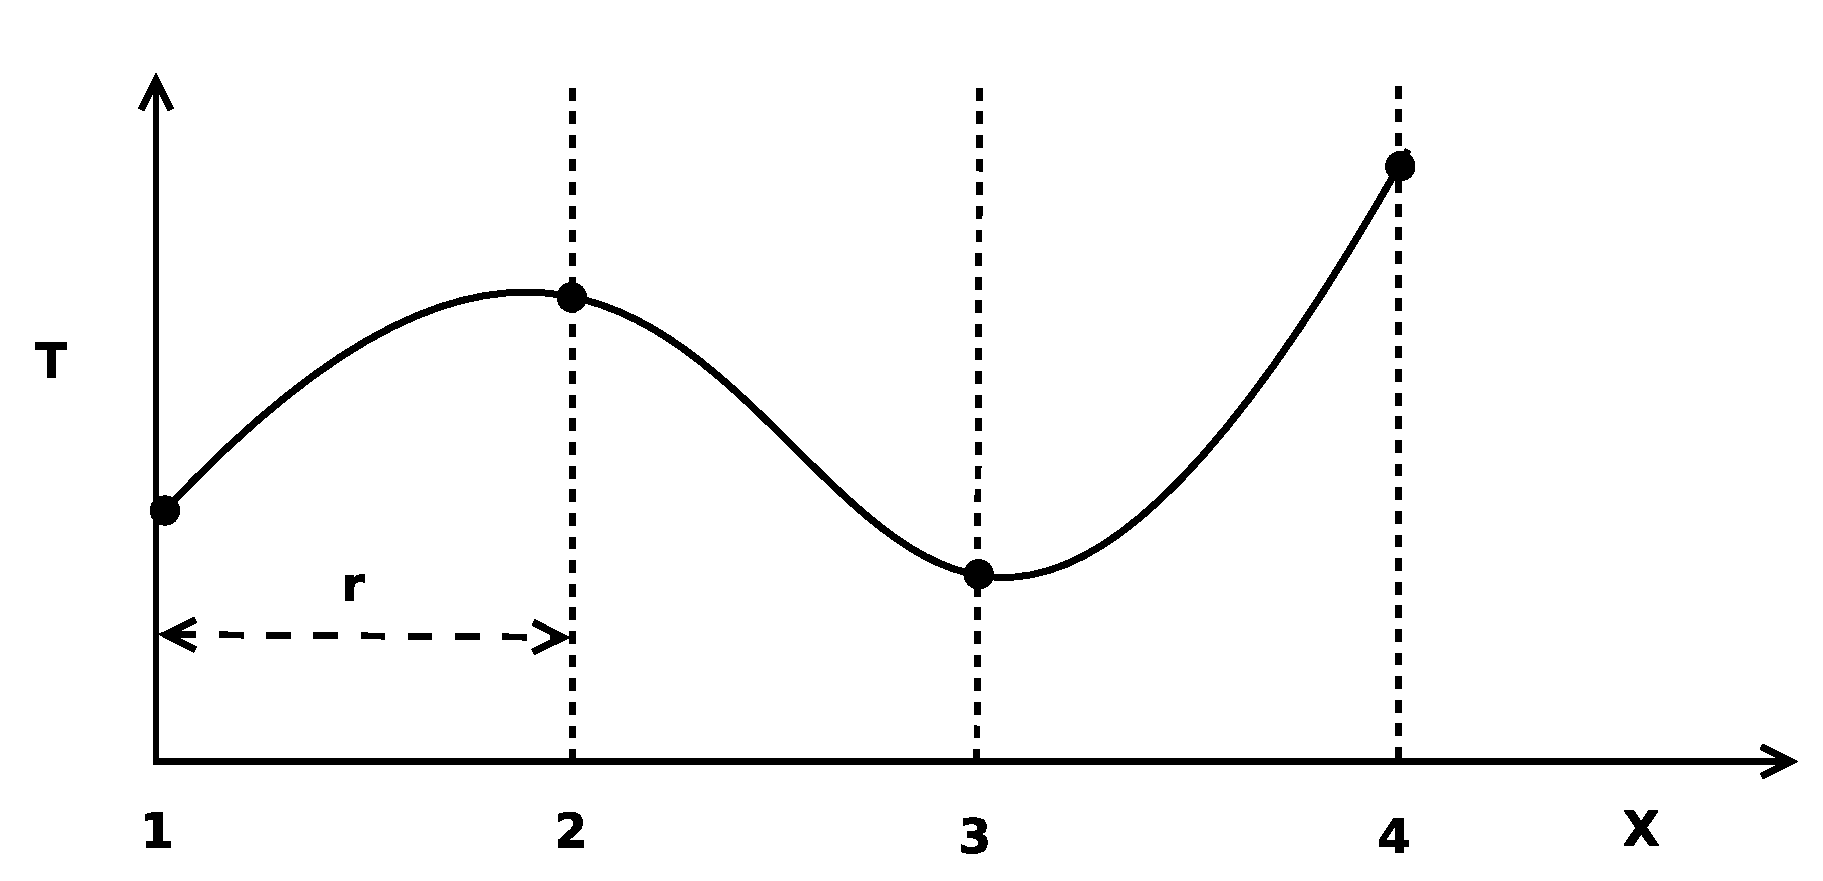
\includegraphics[width=1.0\linewidth]{CG2_2D.eps}
  \caption*{a) Continuous field}
  \label{fig:k0w3}
\end{minipage}%
\begin{minipage}{.5\textwidth}
  \centering
  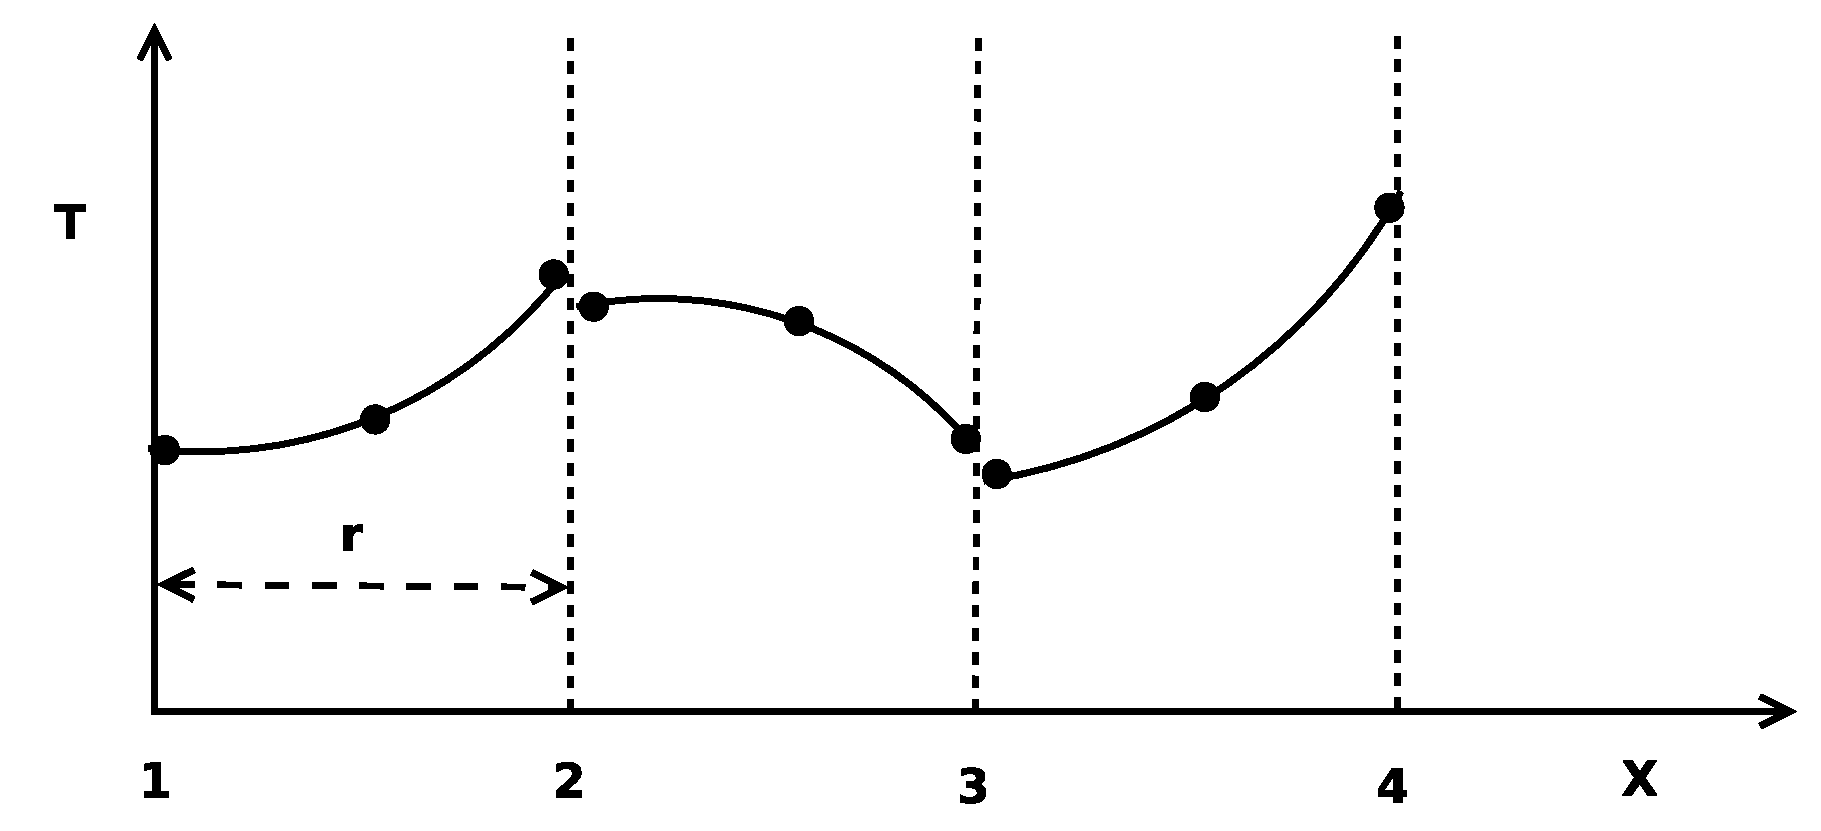
\includegraphics[width=1.0\linewidth]{DG2_2D.eps}
  \caption*{b) Discontinuous field}
  \label{fig:k1w3}
\end{minipage}

\caption{An illustration of a continuous and a discontinuos
  one-dimensional field, showing locations of dofs for each field. The
  continuous field is described by dofs shared between cells.}
\label{fig:differentContinuity1D}
\end{figure}

If a field, or a component of a vector field, is continuous then, as
illustrated, nominally the dofs lie on the mesh entity that is shared
by all the cells through which there exists continuity. 

The pictured location of the degrees of freedom is informative in the
sense that it is easy to understand whether a field is continuous or
discontinuous. It is also informative in the sense that it is easier
to understand which data points are accessed by particular operations
which impacts strategies for carrying out concurrent computations on a
data field. For example, an operation on the dofs in a cell of the
field in Figure~\ref{fig:differentContinuity1D}a affects one of the
edge dofs of each neighbouring cells meaning that these neighbours
cannot be operated on concurrently without risk of data contention
(writing two values to the same edge dof at the same time). Operation
on cells in Figure~\ref{fig:differentContinuity1D}b can all be done
independently and therefore concurrently.

\subsection{Mixed FEM and Order of Basis Functions}
\label{sec:higherOrder}

In a mixed FEM method different discretisations are used to represent
different quantities, and multiple function spaces are therefore
required. In the GungHo dynamical core the main function spaces are
referred to as being {\em mimetic} because the discretisation mimics
desirable properties of the continuous equations. To illustrate, four
of the GungHo function spaces, called ($\mathbb{W}_0$),
($\mathbb{W}_1$), ($\mathbb{W}_2$) and ($\mathbb{W}_3$), are
mathematically related as follows.

\begin{equation}
\begin{array}{ccccccc}
\mathbb{W}_{0} & \overset{\nabla}{\longrightarrow} & \mathbb{W}_{1} & \overset{\nabla\times}{\longrightarrow} & \mathbb{W}_{2} & \overset{\nabla.}{\longrightarrow} & \mathbb{W}_{3}\\
 & \underset{\tilde{\nabla.}}{\dashleftarrow} &  & \underset{\tilde{\nabla}\times}{\dashleftarrow} &  & \underset{\tilde{\nabla}}{\dashleftarrow}
\end{array}\label{eq:derham_complex}
\end{equation}

Additionally, analogous function spaces can be created at {\em lowest
  order} (constant and linear functions) or at increasingly {\em
  higher order} (where constant functions become linear, linear become
quadratic and so forth). Figure~\ref{fig:k0k1w0-w3} shows the dof
placements for the($\mathbb{W}_{0-3}$) functions spaces at lowest
order ($k=0$) and higher order ($k=1$).

The lowest order function spaces all have at most one dof per entity,
and have dofs only on one type of entity. To remember which function
space is which, note that $\mathbb{W}_0$ has dofs on the
zero-dimensional vertices; $\mathbb{W}_1$ has dofs on the
one-dimensional edges, and so forth. 

The $\mathbb{W}_0$ and $\mathbb{W}_3$ function spaces represent mass
fields so the dofs are represented as zero-dimension points in the
figures. The $\mathbb{W}_1$ and $\mathbb{W}_2$ function spaces
represent fluxes so the dofs are represented as a vectors in the
figure.

\begin{figure}
\centering

\begin{minipage}{.5\textwidth}
  \centering
  \includegraphics[width=0.7\linewidth]{k0_W0_dofs.eps}
  \captionof*{figure}{a) $\mathbb{W}_{0}, k = 0$}
%  \label{fig:k0w0}
\end{minipage}%
\begin{minipage}{.5\textwidth}
  \centering
  \includegraphics[width=0.7\linewidth]{k1_W0_dofs.eps}
  \captionof*{figure}{b) $\mathbb{W}_{0}, k = 1$}
%  \label{fig:k0w02}
\end{minipage}

\begin{minipage}{.5\textwidth}
  \centering
  \includegraphics[width=0.7\linewidth]{k0_W1_dofs.eps}
  \captionof*{figure}{c) $\mathbb{W}_{1}, k = 0$}
%  \label{fig:k0w1}
\end{minipage}%
\begin{minipage}{.5\textwidth}
  \centering
  \includegraphics[width=0.7\linewidth]{k1_W1_dofs.eps}
  \captionof*{figure}{d) $\mathbb{W}_{1}, k = 1$}
%  \label{fig:k1w1}
\end{minipage}

\begin{minipage}{.5\textwidth}
  \centering
  \includegraphics[width=0.7\linewidth]{k0_W2_dofs.eps}
  \captionof*{figure}{e) $\mathbb{W}_{2}, k = 0$}
%  \label{fig:k0w2}
\end{minipage}%
\begin{minipage}{.5\textwidth}
  \centering
  \includegraphics[width=0.7\linewidth]{k1_W2_dofs.eps}
  \captionof*{figure}{f)$\mathbb{W}_{2}, k = 1$}
%  \label{fig:k1w2}
\end{minipage}

\begin{minipage}{.5\textwidth}
  \centering
  \includegraphics[width=0.7\linewidth]{k0_W3_dofs.eps}
  \captionof*{figure}{g) $\mathbb{W}_{3}, k = 0$}
%  \label{fig:k0w3}
\end{minipage}%
\begin{minipage}{.5\textwidth}
  \centering
  \includegraphics[width=0.7\linewidth]{k1_W3_dofs.eps}
  \captionof*{figure}{h) $\mathbb{W}_{3}, k = 1$}
%  \label{fig:k1w3}
\end{minipage}


\caption{Locations of dofs for spaces $\mathbb{W}_0$ to $\mathbb{W}_3$
  for lowest order in left column, and next lowest in right. The
  images are not precise enough to show the subtleties of dof
  location. }
\label{fig:k0k1w0-w3}
\end{figure}

There are subtleties about the exact location of the dof. Function
spaces used by GungHo follow the pattern described in
Section~\ref{sec:continuity} where it was stated that a dof can lie on
the entity (face, edge or vertex) across which a field, or component
of the field indicated by the dof, is continuous. But if the field is
discontinuous as it crosses the entity then the cells on each side of
the entity will have their own dof situated on the entity. This is
often illustrated by showing the dof lying very close, but not on, the
shared entity. For example, in Figure~\ref{fig:k0k1w0-w3}~d) the
vertical arrows near each vertex actually lie on the vertical edge,
very close, but not on, the vertex. This is because the dof is shared
with horizontally-neighbouring cells that share the vertical edge, but
not shared with the cells in the layer above or below that share the
vertex. This dof location indicates that the vertical component of the
field is continuous across vertical edges (and faces), but is
discontinuous in the vertical.

In Figure~\ref{fig:k0k1w0-w3}~h) the dofs near the vertices are all
just within the cell, indicating that the field is discontinuous
across all the cell boundaries.

\subsection{Dof-map and data ordering choices}

\subsubsection{Different dof-maps for the same field}

As discussed in Section~\ref{sec:meshSec1} a field array stores the
values for the field, and look-up tables are created to access
sub-sets of values as required by the kernels, such as the subset of
values that are touched by each cell. These look-up tables are
referred to as {\em dof-maps}

In the example shown in Figure~\ref{fig:numberedHexMesh} the look-up
array would be an applicable dof-map for a field with dofs at the
vertices of the mesh. Such a dof-map would be useful when writing a
kernel operation which updates all the vertices on a given cell at
once.

Dof-maps can be set up to list any groupings of dofs. For example, an
application that is set up to ``loop over cells'' will store dof-maps
in which each row lists all the dofs on a cell volume plus the dofs on
the faces, edges and vertices on the boundary of the cell.

If, for reasons of efficiency or easy coding, it is better to loop
over face entities, then a different dof-map would be needed where
each row of the dof-map lists all the dofs of the input field that
contributes to the change in the face dofs of the output field.

\subsubsection{Ordering of data in the field}

Where a field is continuous across a cell boundary and a dofs are,
thereby, shared between entities, the shared dofs will appear in the
dof map of more than one cell. The sharing of dofs has the following
implications for the design of the infrastructure that allows
algorithms to loop over dof-maps.

\begin{itemize}
\item The order in which neighbouring sub-sets of dofs in a dof-map are
  looped over may affect the result of the calculation at the bit
  level because the order in which dofs shared between neighbours are
  updated may change.
\item Where sub-sets of dofs in the dof-map are computed in parallel
  by different shared memory threads then strategies are required to
  prevent two computations updating a shared dof at the same time.
\item Where the global mesh is divided into distributed memory
  parallel domains then some shared dofs at the boundary of the
  domains will, for computational efficiency, exist on two different
  domains. Either, a shared dof should be updated on both domains
  (referred to as redundant computation) or one domain should update
  the shared dof and provide the other domain with the result.
\end{itemize}

\section{PSyKAl}

As discussed in the introduction, PSyKAl is the name for the layered
approach recommended by the GungHo Project and illustrated in
Figure~\ref{fig:psykal}. The PSyKAl approach applies to the scientific
code. The three layers are the Algorithms, the Parallel Systems layer
and the Kernel layer. Scientists write the algorithms and kernels in a
platform-independent manner. The parallel systems layer is the realm
of the software engineer. This section provides a brief overview of
the three layers.

\begin{figure}
\centering
\resizebox{0.66\linewidth}{!}{
\includegraphics*{psykal.ps}}
\caption{Schematic of the GungHo design recommendation illustrating
  the PSyKAl design for the science ``single model'' code, the
  driver layer and supporting infrastructure.}
\label{fig:psykal}
\end{figure}

\subsection{Algorithm layer}

At the Algorithm Layer, scientists write code to operate on full
global fields. {\em DRAFT} Operations may include:

\begin{itemize}
\item Point-wise operations, such as operations to initialise all
  points in a field to a single value, to increment all points in a
  field by a constant amount, or to add or multiply together matching
  points in two different fields.
\item Science operations that operate on one or more fields,
  potentially on different function spaces, on a cell-by-cell
  basis.
\item Operators such as those that transform a field from one
  function space to another.
\end{itemize}

\subsection{Kernels}

Kernels operate on small subsets of the global field. Kernels need to
be designed to get the best out of the future processors that are
envisaged. The optimum size of a kernel (in terms of its memory
footprint and the amount of work it does) will be different on
different architectures.

The GungHo project has recommended that kernels operate on a single
vertical column of data, such as a vertical column of cells. Kernels
will be passed pointers to the field and the dof-map that references
the bottom layer of the column, enabling the kernel to loop over the
whole column by incrementing these references by one for each
level. Ideally, there will be sufficient work to enable the processor
to make use of its vectorising capabilities.

\subsection{Parallel Systems layer}

The Parallel Systems layer (PSy-layer) acts as the interface between
the algorithm layer working on full fields, and the kernel layer which
works on small chunks of the full field. The PSy-layer's job is to
break down the full field into columns and to call the kernels on each
column.

It is intended that the PSy-layer will be created from auto-generated
code. If there is sufficient knowledge about the kernel operations and
the algorithms, the PSy-layer can be generated with appropriate
placement of distributed memory calls to update field halos, and with
loops that use existing shared memory optimisations such as OpenMP or
OpenACC.

It is intended that the tools that generate the PSy-layer code will be
adaptable to different architectures.

\section{Dynamo}
\subsection{Introduction}

Dynamo is an application that comprises the Met Office implementation
of the GungHo dynamical core. It is being developed in a collaboration
between the Met Office, STFC, and Manchester University with input and
advice from other GungHo partners. The following sections describe
some of the technical details of key parts of the Dynamo
implementation, and relate these details to aspects of the GungHo
design described above.

The GungHo dynamics can be implemented with different choices of mesh
topology and order of the finite element method, and it is possible
that future dynamical cores will employ a different choice of function
space. Dynamo is designed to be adaptable to changes in these
assumptions. 

Dynamo is currently under develoment and this is indicated by the fact
that some of the following sections describe features that are not yet
complete. These are marked with ``TBD'' - To Be Done.

Dynamo is written in Fortran 2003 and uses several object-oriented
features of Fortran 2003.

\subsubsection{Overview}

The design of Dynamo science codes follows the PSyKAl design
(Figure~\ref{fig:psykal}) that imposes a ``separation of concerns''
between scientists writing science algorithms and kernels and software
developers maintaining the infrastructure and the parallel systems
layer that ensures the code runs efficiently on different
supercomputers.

The Dynamo data model supports the PSyKAl separation of concerns by
providing appropriately designed objects and coding standards.

The Dynamo data model enables fields to be created within scientific
``Algorithm'' code on one of a choice of function spaces. The choice
of function spaces in a given release of Dynamo is fixed, but the
Dynamo design is intended to make it easy to add new function spaces.

Each function space is related to a mesh. Currently a given
configuration of Dynamo has only one mesh. Support will be added later
for hierarchies of meshes (such as lower resolution versions of a
mesh). Such mesh hierarchies will support a multigrid-based solver and
enable the physics components to use a different resolution to the
dynamics while ensuring that coupling between the two does not involve
complex interpolation.

Fields can be created with one or more levels. However, all fields in
a given deployment of Dynamo currently have the same number of levels.

Dynamo can be configured to use several different meshes all based on
quadrilateral cells. Options include a spherical mesh such as a cubed
sphere, a biperiodic mesh, and a ``trench'' mesh (one which is
periodic in one dimension). Dynamo supports distributed memory
deployment by decomposing the full ``global'' mesh into local meshes
for each rank.

In the algorithm layer, scientists write code to operate on whole
fields. This is done by calling an {\tt invoke} subroutine with the
names of kernels or operations and lists of fields and scalars to be
passed to each kernel and operation.

The invoke interface is not a real Fortran interface. The PSy-layer
code is auto-generated by a tool called PSyclone. It generates a
subroutine call for each call to {\tt invoke} in the algorithm
layer. The PSyclone tool modifies the algorithm code to change the
call to {\tt invoke} into a call to the generated subroutine.

The PSy-layer subroutines are primarily based on the metadata in the
kernels referenced by the invoke subroutine call, and a script that
defines optimisations to be applied to the code. The subroutines
extract the necessary information required to address and understand
the fields. They call the kernels with data from the field, one column
of data per call. 

Dynamo supports a semi-unstructured mesh and a range of different
function spaces. Operations on fields are supported by appropriate
dof-maps that allow the PSy-layer to loop over all the data in the
fields.

Field data in memory are structured with the levels index
inner-most. This means that dof-maps only need to address the cells in
the first level of a 3D field. Kernels loop through the column of data
by operating first on the cell addressed by the dof map, and looping
through the column of cells by adding one to the address of each dof
to address the equivalent dofs on each subsequent level.

The PSyclone tool generates code within the PSy-layer subroutines that
supports distributed memory deployment of Dynamo by including
appropriate calls to update halo cells when appropriate. For example,
updates need to be called on fields whose halos are modified by kernel
calls if the field is subsequently provided as an input to another
kernel call.

The PSyclone tool constructs code that uses shared memory optimisation
techniques as appropriate. Currently, OpenMP is supported. Shared
memory optimisations need to consider ``colouring'' of the domain so
that two operations that act on one data point are not done
concurrently, and are done in a reproducible order that preserves bit
comparison. Colour maps are generated for the mesh and accessible
through operations on the field.

TBD later Further, by identifying independent kernel calls within a
given invoke call, PSyclone can generate code that will call these
kernels concurrently. This technique is called ``loop fusion''. Dynamo
orders data in the fields that allow cells affected by distributed
memory halo updates to be operated on in separate loops from
operations on the core field. In future, PSyclone will support
concurrent communication and computation, where halo operations occur
while cells on the core field are operated on.

The PSy-layer contains code that loop over cells owned by the local
domain, not the halo cells. Some kernels require stencil data -- input
data from neighbouring cells. PSyclone constructs stencil maps from
the dof-maps to provide to the kernel.

Currently, the halo in Dynamo is hard-wired to fulfil the needs of the
largest required stencil. TBD Dynamo could be refined to create halos
for each specific requirement:- either different halos for different
function spaces or, going further, different halos for different
fields.

Given that kernels will loop over all the cells in a local domain,
updates to dofs that exist on the boundary between two or more
distributed memory regions will be redundantly computed on all ranks
that cover these regions.

\subsection{Mesh and connectivity}

On starting, Dynamo reads a mesh description of a 2D mesh from a UGRID
netCDF file. This mesh description is referred to as a ``global''
mesh. The name ``global'' means it is the full mesh, not necessarily a
mesh that covers the whole globe of the Earth. By contrast, the
``local'' meshes are created for each partition of a distributed
memory configuration. 

Information about the global mesh includes coordinates of vertices,
and connectivity information. Connectivity information includes vertex
to vertex connectivity (which defines edges of the 2D cells) and cell
to vertex connectivity. The ordering of the coordinate and
connectivity information specifies a global numbering of each of the
entity types.

The topology of a reference element, a unit cell, is required to
enable consistent understanding of function spaces throughout the
code. Information about the reference cell includes an ordered list of
the coordinates of the vertices, an ordered list of the faces and
edges for the cell, connectivity information between the different
entities, and some geometry information.

Dynamo includes a definition of a reference cell for a cube and a
triangular prism.

\subsection{Partitions and halos}

\begin{figure}
\centering

\begin{minipage}{.4\textwidth}
  \centering
  \includegraphics[width=0.7\linewidth]{partitioning1.1.eps}
  \caption*{a) A part of a global 2D mesh with global cell numbering}
  \label{fig:global}
\end{minipage}%
\begin{minipage}{.4\textwidth}
  \centering
  \includegraphics[width=0.7\linewidth]{partitioning2.eps}
  \caption*{b) The partitioned mesh with global cell numbering and halos. Core
    cells are white; owned cells are light grey; halos are dark grey.}
  \label{fig:partitioning_cells}
\end{minipage}

\begin{minipage}{.4\textwidth}
  \centering
  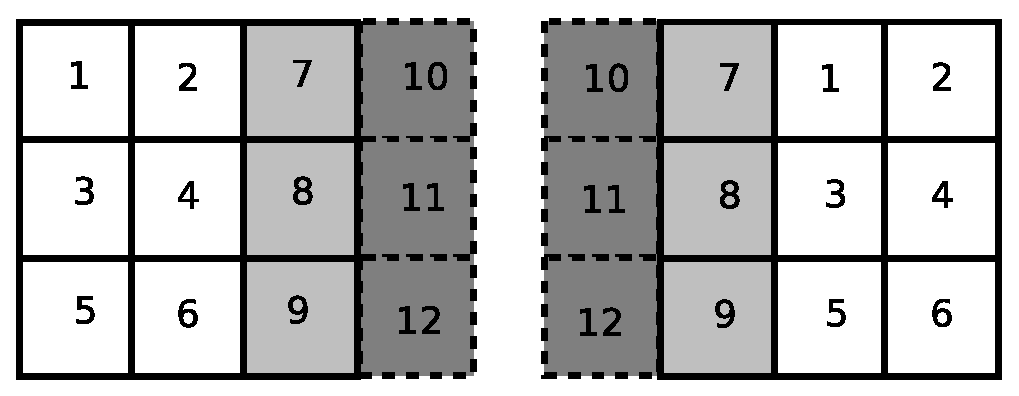
\includegraphics[width=0.7\linewidth]{partitioning3.eps}
  \caption*{c) Cells in each partition are locally numbered -- core
    cells are numbered first followed by owned then halo cells.}
  \label{fig:local_number}
\end{minipage}%
\begin{minipage}{.4\textwidth}
  \centering
  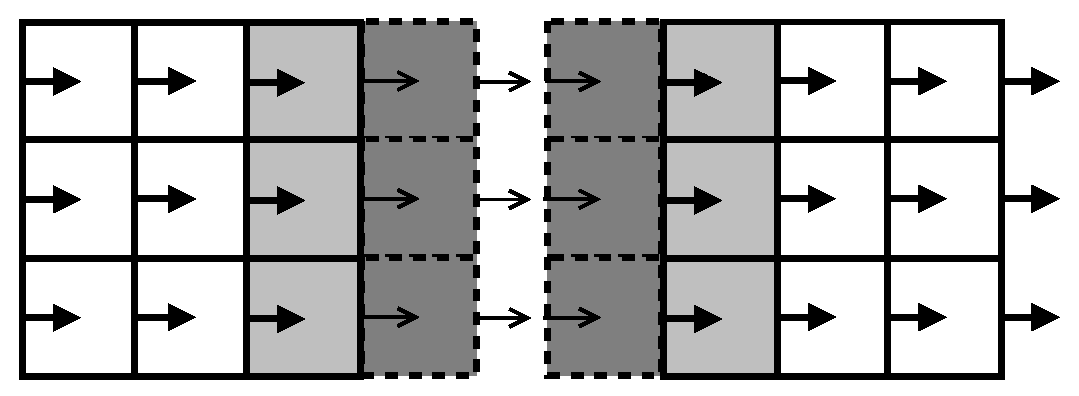
\includegraphics[width=0.7\linewidth]{partitioning4.eps}
  \caption*{b) Ownership of dofs on cell edges and vertices has to be
    decided. In this case, the arrows indicate dofs on the cell
    edge. The wide arrows are owned or core dofs. The narrow arrows
    are halo dofs. The edge between the two partitions (indicated by
    the edge between the owned and halo cells on each partition) is
    owned by the right-hand rank.}
  \label{fig:partitioning_dofs}
\end{minipage}

\end{figure}

TBD: Update in relation to inner halos is required.

Each distributed memory rank creates a local mesh based on the global
mesh and a partition strategy. The partition strategy is mesh-type
dependent in that specific strategies are provided to support a
cubed-sphere mesh and a biperiodic mesh. TBD further mesh partition
strategies can be added, including addition of a generic mesh
partitioner.

The partition strategy is stored within a partition object - see
Section~\ref{sec:partition_class}

The partitioning of the global mesh between distributed memory ranks
is based around partitioning of the cell entities of the 2D mesh, and
extruding the local 2D partition.  Based on the number of distributed
memory ranks and the chosen partition strategy, each rank computes a
local partition of cells and then creates a 3D mesh by extruding the
2D mesh into the vertical.

Based on the stencil requirements of the model kernels, each rank
computes a set of halo cells. Currently, the halo size is hard-wired
to a single fixed value for all field types according to the needs of
kernels that currently exist in the Dynamo implementation of
GungHo. TBD In the future, the halo size of a given field will be
dependent on the specific requirements of the kernels.

Having computed the set of cells in the local partition with halos the
sets of cells are ordered as follows:

\begin{itemize}
\item Core cells: cells that are not in the halo of any other rank.
\item Owned cells: cells that are owned by the local partition, but
  that are in the halo of another rank.
\item Halo cells.
\end{itemize}

To support concurrent computation within a shared memory domain, the
mesh needs to be ``coloured''. Colouring involves dividing the mesh
into sub-groups of cells and giving each sub-group a nominal
colour. The degrees of freedom associated with the cells of a given
colour subgroup are independent of all other cells of the same
colour. Therefore, if operations on all cells of the same colour take
place concurrently, the results of one operation do not overwrite the
results of another.

\subsubsection{The Partition Class}

\label{sec:partition_class}

The partition class provides a set of functions to partition a global
2D mesh and to access information about the local partition such as
the range of cells in the core of the partition or in the halo. Such
information can be used by PSyclone to break down the processing of
data into, for example, loops over cells that are unaffected by
distributed memory communications and loops over cells, such as halo
cells, that are. This would allow strategies such as concurrent
communication and computation to be applied.

Also included in the partition class are functions required to manage
distributed memory communications such as those used to relate the
local cell number and global cell number, and functions that return
information about the local distributed memory rank number and the
total number of ranks.

\subsection{Declaring Fields}

Once the mesh setup is complete, scientific fields can be
declared. Fields are declared on one of a fixed choice of function
spaces. A function space instance for a particular function space type
is created only if a field on that function space is created. The same
function space instance is then used by subsequent fields created
using the same function space type.

\subsubsection{Function Space definitions and dof-maps}

A given scientific formulation such as GungHo requires a certain set
of function spaces. Some of the GungHo function spaces
($\mathbb{W}_{0-3}$) are illustrated in
Figure~\ref{fig:k0k1w0-w3}. The class {\tt function\_space\_type} is
used to construct instances of each function space required.

The function space instance is created on demand the first time a
field on that function space is requested. Additional fields of the
same type use the same function space instance. The function space
instance is created for a given mesh instance and a given order. Each
distributed memory rank creates a function space instance for its own
local partition.

Information in the function space instance includes:

\begin{itemize}
\item The dof-map for the first level of cells of the 3D mesh.
\item the number and location of degrees of freedom within the whole
  3-dimensional extent of the local mesh.
\item Functions to evaluate the basis functions.
\item Functions to access the range of dofs in different parts of the
  local field, such as those within a given halo.
\item Functions to access information about the mesh, such as its
  colouring strategy.
\end{itemize}

The function space instance defines the order of storage of dofs in
the local 3D field. Essentially, dofs are ordered with the core dofs
first: core dofs are those that are not represented in the core or
halo of any other rank. Following the core cells, dofs are arranged in
halo order, from inner to outer. 

This ordering supports two things:

\begin{itemize}
\item Computation of the core cells can be done concurrently with
  updating of any of the halo cells.
\item Exchange of halo cells involves sending and updating arrays of
  data that are contiguous in memory.
\end{itemize}

\subsubsection{Fields and Field Proxies}

\label{sec:proxy}

A field is created for a given function space. A typical operation to
create a new field at the algorithm level is as follows.

\begin{verbatim}
   theta = field_type(vector_space = function_space%get_instance(mesh, W0))
\end{verbatim}

The field type contains various operations that can take place on the
field data, but does not actually allow access to the data itself as
the data is held privately. A {\tt field\_proxy} type provides functions
that allow access to the field data and the dof-maps.

Coding rules for Dynamo require that {\tt field\_proxy} types cannot
be accessed in the algorithm layer. Only the PSy-layer can access {\tt
  field\_proxy} types. These rules mean that algorithms only operate
on fields as a whole and not on individual data points.

The {\tt field\_proxy} type allows access to the data, and to
distributed memory operations on the data such as halo exchange
operations and global sums.

\subsection{Quadrature Rules}

A quadrature rule is an approximation of the integral of a function
based on a weighted sum of values at a range of points. Dynamo kernels
specify the type of quadrature rule in its metadata.

The precise quadrature rule is defined by the algorithm and passed as
an argument to the {\tt invoke} interface.

\begin{verbatim}
  type( quadrature_type) :: qr
  qr = quadrature_type(element_order+3, GAUSSIAN)
...
  call invoke( compute_grad_operator_kernel_type(grad, chi, qr) )
\end{verbatim}

The PSy-layer dereferences the values required to apply the quadrature
rule and passes them to the kernel.

\subsection{Driver and Algorithm level}

The algorithm layer is the layer where high level abstractions of
algorithms employed in Dynamo are written by scientists. Operations
are defined in terms of whole fields, there are no references to
particular geographical locations, or cell array indices. The
algorithm layer can operate on fields in the following way:

\begin{itemize}
\item Kernel operations: Kernels operate on a whole field. They take
  arguments of one or more fields and return a single updated field.
\item Inner product operations. These take fields as arguments and
  return a scalar
\item Point-wise operations. Point-wise operations act on dofs
  individually. For example, to initialise all values of a field to a
  constant, or to add two fields together.
\end{itemize}

At the algorithm (and driver) level, a scientist needs to create field
instances, initialise their data, and to call operations that act on
the field data. The algorithm can also specify the quadrature rule
that should be used by the kernel.

\subsection{The {\tt invoke} interface}

\label{sec:invoke}

Calls by the algorithm to carry out operations on fields are requested
by calling the {\tt invoke} subroutine.  The {\tt invoke} subroutine
does not actually exist in the final executable. At build time, prior
to compilation the algorithm layer code is modified such that each
call to {\tt invoke} is changed to be a call to an
automatically-generated PSy-layer subroutine or to a subroutine that
is part of the Dynamo infrastructure.

\subsubsection{Kernel Operations}

Kernel subroutines update the values of an output cell of a field
based on the input cells from one or more fields plus optional stencil
cells, or based on an operator. The {\tt invoke} subroutine call
includes arguments comprising a list of kernel constructors. Each
kernel constructor takes a list of arguments that can comprise input
and output fields, scalars and a quadrature rule, or operators.

The PSy-layer generates a subroutine call for each {\tt invoke} that
takes all the arguments of all the kernel constructors listed in the
{\tt invoke} call.

\begin{verbatim}
call invoke(rtheta_kernel_type(rtheta, u, chi, qr1), kernel2_type(field3, qr2))
\end{verbatim}

The kernel subroutine in kernel module {\tt rtheta\_kernel\_type}
takes two fields {\tt u} and {\tt rtheta}, the coordinate field {\tt
  chi}, and one quadrature rule as its input arguments. The kernel
subroutine in kernel module {\tt kernel2\_type} takes one field and a
different quadrature rule as its input.

The {\tt invoke} interface can take one or more kernel constructor as
an argument. Scientists should combine multiple kernels together where
the separate kernels can be invoked independently of each other. This
enables the system to optimise the model by running kernel operations
in parallel where appropriate.

\subsubsection{Operator Kernels}

Operator kernels create operators such as grad, div and curl, that can
be used to operate on fields through calls to other kernels.

\subsubsection{Point-wise operations}

Point-wise operations are operations that can be or need to be
computed by directly accessing each dof rather than using the dof-map
to indirectly address the dofs. Dynamo provides specific subroutine
interfaces for each point-wise operation required. Each one takes
fields and scalars as arguments and returns a field or a scalar.

TBD. PSyclone is adding support to generate pointwise
operations. Pointwise operations will then be called using the {\tt
  invoke} interface as for current kernels, but there will be no
kernel code in Dynamo.

Example point-wise kernels include operations to initialise a field to
a fixed value and operations to compute inner products.

\subsection{PSy-layer}

The Parallel Systems layer, or PSy-layer, contains subroutines that
fulfil the field operations requested by the algorithm layer.  The PSy
layer holds the code that implements parallelism within science model
code. The PSy-layer code is largely generated by the PSyclone
tool. Dynamo supports fixed PSy-layer code for kernel requirements
that are not met by PSyclone. However, it is intended that
hand-written PSy-layer code is an interim solution that needs to be
met by enhancements to the PSyclone tool.

The PSy-layer subroutines access field data, dof-maps, and information
about the quadrature rules required to run the kernel operations on
the input data. Specifically, the subroutines loop over the relevant
dof-maps and call the kernel once on each cell.

PSy-layer code generation is based on the metadata descriptions in the
kernel object. The kernel metadata lists, for example, the function
space of each field, whether the field is an input or output, whether
the kernel requires a stencil (TBD) and which entity the kernel loops
over (currently looping over cells is supported).

Additionally, the PSyclone tool is designed to correctly implement
shared memory optimisations such as OpenMP, and to correctly place
calls to distributed memory routines to update halos.

Where a kernel or field operation is required that is not supported by
the PSyclone tool, PSy-layer code can be hand-written. Such code is
referred to as ``PSyKAl-lite'' code.

PSyclone is documented elsewhere.

\subsubsection{Kernels}

Kernels process a single vertical column of field data from one or
more fields. A vertical column comprises the column of dofs relating
to a single row of any one of the dof-maps that have been generated
(for example to facilitate looping over cells or over faces).

A kernel type definition contains metadata describing the inputs it
requires in sufficient detail to enable the PSy-layer code to be
correctly written. For example, in the following kernel, the {\tt
  meta\_args} setting means that the kernel takes 5 field
arguments. The first argument is the output field as defined by the
{\tt GH\_INC} increment tag. The remaining arguments are input
arguments. The last argument is an array of 3 fields (in this case it
is the coordinates of the mesh vertices). The {\tt W0} to {\tt W3}
settings describe the function space of each field.

The {\tt meta\_funcs} definition describes the quadrature rule to use
for each function space. 

\begin{verbatim}
type, public, extends(kernel_type) :: vorticity_advection_kernel_type
  private
  type(arg_type) :: meta_args(5) = (/                                  &
       arg_type(GH_FIELD,   GH_INC,  W2),                              &
       arg_type(GH_FIELD,   GH_READ, W2),                              &
       arg_type(GH_FIELD,   GH_READ, W3),                              &
       arg_type(GH_FIELD,   GH_READ, W1),                              &
       arg_type(GH_FIELD*3, GH_READ, W0)                               &
       /)
  type(func_type) :: meta_funcs(4) = (/                                &
       func_type(W2, GH_BASIS),                                        &
       func_type(W3, GH_BASIS),                                        &
       func_type(W1, GH_BASIS),                                        &
       func_type(W0, GH_DIFF_BASIS)                                    &
       /)
  integer :: iterates_over = CELLS
contains
  procedure, nopass ::vorticity_advection_code
end type
\end{verbatim}

Kernels that require stencils will have additional metadata describing
the stencil requirement.

\begin{verbatim}
DRAFT: Detail TBD
type, public, extends(kernel_type) :: kernel_with_stencil_kernel_type
  private
  type(stencil_dofmap_type) :: meta_stencil(2) = (/    &
       stencil_dofmap_type(STENCIL_POINT),             &
       stencil_dofmap_type(STENCIL_1DX, 2),            &
       /)
...
end type
\end{verbatim}

The following is an example kernel subroutine based on the {\tt
  rtheta\_kernel\_type} invocation described in
Section~\ref{sec:invoke}.

The subroutine has a much longer argument list than the {\tt invoke}
call in the algorithm layer. The input arguments are satisified by
code in the PSy-layer that creates pointers to data in proxy objects
(see Section~\ref{sec:proxy} that are visible only to the PSy-layer
and not to the algorithm layer.  They include references to dof-maps
that point to the dofs in the input fields, the number of layers in
the fields, the basis functions and basis function differentials, the
number of quadrature points in the quadrature rule, and the weights.

Within the kernel the main loop is over nlayers of the column of a
cell of the input field dofs as referenced by the cell dof-maps {\tt
  map\_w0} and {\tt map\_w2}.

\begin{verbatim}
module rtheta_kernel_mod
use kernel_mod,              only : kernel_type

<snip>---------------

contains
! rtheta_kernel_code: The subroutine which is called directly by the Psy layer
! nlayers: the number of layers
! ndf_w0/2: The number of degrees of freedom per cell for w0/w2
! map_w0/2: Arrays holding the dofmaps of the cell at the base of the column for w0/w2
! w0_basis: Array holding basis functions evaluated at quadrature points 
! w0_diff_basis: Differential of the basis functions evaluated at quadrature points 
! r_theta: Output data field
! chi_1/2/3: The x,y,z Cartesian coordinate in w0
! u: Input data field - the velocity
! nqp_h, nqp_v: Number of quadrature points in the horizontal and vertical
! wqp_h, wqp_v: 1-d array of horizontal/vertical quadrature weights

subroutine rtheta_kernel_code(nlayers,                                         &
                       ndf_w0, undf_w0, map_w0, w0_basis,  r_theta,            &
                       ndf_w2, undf_w2, map_w2, w2_basis, orientation, u,      &
                       w0_diff_basis, chi_1, chi_2, chi_3,                     &
                       nqp_h, nqp_v, wqp_h, wqp_v )
                               
  ! Arguments
  ! Cell dof-maps for base of w0 and w2 column
  integer, dimension(ndf_w0), intent(in) :: map_w0
  integer, dimension(ndf_w2), intent(in) :: map_w2

  ! Basis function fields
  real(kind=r_def), dimension(1,ndf_w0,nqp_h,nqp_v), intent(in) :: w0_basis  
  real(kind=r_def), dimension(3,ndf_w0,nqp_h,nqp_v), intent(in) :: w0_diff_basis  
  real(kind=r_def), dimension(3,ndf_w2,nqp_h,nqp_v), intent(in) :: w2_basis 

  ! Full field for the local rank
  real(kind=r_def), dimension(undf_w0), intent(inout) :: r_theta
  real(kind=r_def), dimension(undf_w0), intent(in)    :: chi_1, chi_2, chi_3
  real(kind=r_def), dimension(undf_w2), intent(in)    :: u

<snip>---------------

  ! Loop over layers
  do k = 0, nlayers-1
  ! Extract element arrays of chi
    do df = 1, ndf_w0
      loc = map_w0(df) + k ! Create a dof-map for the cell on level (k+1)
      chi_1_e(df) = chi_1( loc )
      chi_2_e(df) = chi_2( loc )
      chi_3_e(df) = chi_3( loc )
      rtheta_e(df) = 0.0_r_def
    end do
    call coordinate_jacobian(ndf_w0, nqp_h, nqp_v, chi_1_e, chi_2_e, chi_3_e,  &
                             w0_diff_basis, jac, dj)
<snip>---------------
  ! compute the RHS integrated over one cell
    do qp2 = 1, nqp_v
      do qp1 = 1, nqp_h
        u_at_quad(:) = 0.0_r_def
        do df = 1, ndf_w2
          u_at_quad(:)  = u_at_quad(:)  + u_e(df)*w2_basis(:,df,qp1,qp2)
        end do
<snip>---------------
      end do
    end do
  end do
end subroutine rtheta_code

\end{verbatim}

\begin{thebibliography}{9}

\bibitem{buckeridge}
  S. Buckeridge and R. Scheichl,
  \emph{Parallel geometric multigrid for global weather prediction},
  Numer. Linear Algebra,
  17(2-3),
  2010.

\bibitem{macdonald}
  A.E.~MacDonald, J. Middlecoff, T. Henderson, and J.L. Lee
  \emph{A general method for modeling on irregular grids},
  International Journal of High Performance Computing Applications,
  25(4),
  2011.

\bibitem{gunghocs}
  R.~Ford et al.
  \emph{GungHo Phase 1: Computational Science Recommendations
A general method for modeling on irregular grids},
  Met Office Forecasting Research Technical Report No: 587,
  2013.

\end{thebibliography}

\end{document}
